\documentclass{ecai}
\usepackage{graphicx}
\usepackage{latexsym}

\ecaisubmission   
% inserts page numbers. Use only for submission of paper.
                  % Do NOT use for camera-ready version of paper.

\usepackage{amsmath}
\usepackage{amsthm}
\usepackage{algorithm}
\usepackage{algorithmic}


\begin{document}

\begin{frontmatter}

\title{Contrastive Highlights: Explaining Reinforcement Learning Policies via Outcomes}

% \author{\fnms{Yael}~\snm{Septon}\orcid{0000-0002-2798-990X}\thanks{Corresponding Author. Email: yael123@campus.technion.ac.il}}
% \author{\fnms{Yotam}~\snm{Amitai}\orcid{0000-0002-0084-9739}}
% \author{\fnms{Ofra}~\snm{Amir}\orcid{0000-0003-2303-3684}} 
% \address{Technion, Faculty of Data \& Decision Science}


\begin{abstract}
Explainable reinforcement learning (XRL) methods aim to help elucidate agent policies and their underlying decision-making processes. The majority of XRL approaches focus on local explanations, seeking to shed light on the reasons an agent acts the way it does at a specific world state. While such explanations are both useful and necessary, they often fail to account for the outcomes of the agent's selected choice of action, i.e., they portray the agent's reasoning but not its manifestation. 
In this work, we propose ``contrastive highlights'', a new local explanation method that visually compares the agent's chosen behavior to an alternative choice of action in a contrastive manner. This approach demonstrates alternative trajectories the agent could have taken, and can be complementary to other local explanation methods. 
We conducted user studies to evaluate the usefulness of contrastive highlights in supporting people's understanding of agents' preferences. We compared contrastive highlights with reward decomposition,  a local explanation method that presents an agent's expected utility for different actions by decomposing it into meaningful reward types. We further examined the integration of reward decomposition with contrastive highlights.
Our results show that integrating reward decomposition with contrastive highlights significantly improved participants' performance compared to using each of the approaches separately.
\end{abstract}

\end{frontmatter}

\section{Introduction}
The behavior of reinforcement learning (RL) agents is complex - these agents operate in large, stochastic settings, and are trained through rewards received during their interaction with the environment, which is often sparse. Moreover, state-of-the-art RL models often utilize deep learning, resulting in complex models that can be hard to interpret, making the task of explaining such an agent's behavior even more complicated. While supporting people's understanding of the decision-making of RL agents is challenging, it is important for facilitating effective collaboration and appropriate trust, in particular in high-stakes domains~\cite{2210.11584} such as healthcare or transportation. 

%state of the art
Numerous approaches for explainable reinforcement learning (XRL) have been proposed in recent years \cite{milani2022survey}. Some methods aim to explain \emph{local} decisions of the agents in particular world-states. These include saliency maps that show what features of the state the agent attends to \cite{greydanus2017visualizing}, causal action graphs \cite{madumal2020explainable} that are based on a causal model of the agent's policy, or reward decomposition \cite{juozapaitis2019explainable} which depict the agent's expected reward for different components of the reward function, among others. In contrast to these local explanation methods, a complementary set of explanation approaches aim to convey the \emph{global} policy of the agent, that is, describe its overall strategy, behavior, or how it behaves in different regions of the state space. Such approaches include policy summaries \cite{amir2019summarizing} that demonstrate the behavior of the agent in a selected set of world-states based on some criteria or learning a decision tree that corresponds to the agent's policy \cite{liu2018toward}. 


% what's new and why
In this work, we focus on helping laypeople understand and anticipate agent preferences by depicting the trade-offs between alternative actions. We propose a new method for visualizing the outcomes of actions \textit{not} taken by the agent as a means to explain their chosen action. We introduce ``contrastive highlights'', a new local explanation method that draws inspiration from global policy summaries~\cite{amir2019summarizing} while focusing on a local decision -- which action to take in state $s$. Similar to policy summaries, contrastive highlights convey agent behavior by showing trajectories of the agent acting in the environment. However, while policy summaries only show the actions chosen by the agent, contrastive highlights exhibits both the trajectory beginning with the chosen action, as well as a simulated \emph{contrastive} trajectory showing its course had it chosen a different action in the same world-state. By displaying the outcomes of both actions side-by-side, contrastive highlights aims to provide more information regarding the decision made by the agent. Our hypothesis is that observing the outcomes (“what if?”) is beneficial to users wishing to understand the agent’s behavior and recognize agent preferences. The contrastive nature of the explanation is in line with the literature on explanation in the social sciences which show that people typically provide and prefer explanations that contrast alternatives \cite{miller2019explanation}. Additionally, contrastive highlights can be integrated into policy summaries, and can also complement other local explanation methods. In particular, this approach naturally complements methods that present the agent’s \textit{motivation} for choosing a specific action (“why?”), such as \textit{reward decomposition}~\cite{juozapaitis2019explainable} which quantifies the agent's expectations regarding the utility of different actions. 


% results
To evaluate the contribution of contrastive highlights to people's understanding of agents' preferences, we conducted two user studies. Participants were presented with explanations in the form of contrastive highlights, reward decomposition, or a combination of both. Based on these explanations, participants were asked to characterize the reward function of the agent by ranking its preferences. Both studies showed that combining reward decomposition with contrastive highlights improved participants' understanding, compared to showing only one of the explanations. 

Our contributions are threefold: 
\begin{enumerate}
\item We introduce contrastive highlights, a new local explanation method for highlighting trade-offs between alternative courses of actions that an agent considers. 

\item We integrate contrastive highlights with reward decomposition to provide users with both a quantification of the expected utility of actions as well as with a visualization of alternative outcomes given a different choice of actions.

\item We propose a way to generate global explanations augmented by contrastive highlights which selects summary states based on a contrast measure.

\item We conduct user studies showing both that our new method is beneficial as of itself, and that its integration with reward decomposition results in greater performance and understanding of agent behavior compared to each method separately.
\end{enumerate}

\section{Related Work}
Our work is motivated and draws inspiration from \emph{global} RL explanation approaches. These approaches aim to provide users with a higher-level description of the agent by attempting to portray its behavior, strategy, capabilities, or logic ~\cite{huang2019enabling,amir2019summarizing,booth2019evaluating}. 

One approach for conveying the global behavior of an agent is \emph{Agent Strategy Summarization} ~\cite{amir2019summarizing}. In this paradigm, the agent's policy is demonstrated through a carefully selected set of world states. The strategy summarization objective is to select the subset of state-action pairs that best describes the policy of the agent. Formally, Amir \& Amir~\cite{amir2018highlights} defined the set $T= <t_1,...,t_k>$ as the trajectories that are included in the summary. A Trajectory is composed of a sequence of $l$ consecutive states and the actions taken in those states, $<(s_i,a_i),...,(s_{i+l-1},a_{i+l-1})>$. 
The criteria for selecting states can vary based on the summary objective, e.g., state importance \cite{amir2018highlights,sequeira2020interestingness,huber2021local} or using machine teaching approaches~\cite{lage2019exploring,huang2019enabling}.

Building upon this approach, the DISAGREEMENTS algorithm ~\cite{amitai2021don} portrays the diverging trajectories of two agents upon reaching a disagreement between them on how best to proceed from a given state. It provides a  side-by-side comparison of the difference in outcomes between the agents, constituting a method for agent comparison and behavior difference evaluation.
The contrastive highlights method proposed in this paper builds on and extends the DISAGREEMENTS algorithm both for the single-agent use case and for generating a \emph{local} explanation.

Local explanations in XRL seek to describe why a particular choice of action was made by a given agent in a specific world-state~\cite{tabrez2019explanation,dodson2011natural}, for example by using saliency maps to identify what elements of the environment the agent pays attention to~\cite{hilton2020understanding,huber2019,puri2020} or generating causal explanations by constructing the agent's action graph~\cite{madumal2020distal}.
Many RL methods make use of the agent's learned Q-values for selecting the optimal action in a given state. While useful for evaluating expected utility, it does not provide any information as to what factors contributed to the agent's preference for one action over another. Juozapaitis et al.~\cite{juozapaitis2019explainable} made use of reward decomposition to obtain insights into these factors. Decomposing the environment's reward into a sum of meaningful reward types enables to provide explanations on which action has an `advantage' over other actions. 

Anderson et al.~\cite{anderson2019explaining}
present a user study that investigates the impact of explanations on non-experts' understanding of reinforcement learning agents. They investigate both a common RL visualization, saliency maps, and reward decomposition bars. They designed a four-treatment experiment to compare participants' mental models of an RL agent in a simple Real-Time Strategy game. Their results showed that the combination of both saliency and reward bars was needed to achieve a statistically significant improvement in the mental model score over the control.

In this work, we suggest a new local explanation method and focus on reward decomposition as a baseline for comparison and as well as showing how our method can be integrated with it. We chose to focus on reward decomposition rather than saliency maps as the baseline method since reward decomposition provides an intrinsic explanation (i.e., it describes the actual model) and because there is evidence that laypeople have difficulty interpreting saliency maps~\cite{huber2021local}.
 

% \subsection{Global Explanations}
% Global explanations provide a higher-level description of the agent by attempting to portray its behavior, strategy, capabilities, or logic ~\cite{huang2019enabling,amir2019summarizing,booth2019evaluating}. 

% One approach for conveying the global behavior of an agent is \emph{Agent Strategy Summarization} ~\cite{amir2019summarizing}. In this paradigm, the agent's policy is demonstrated through a carefully selected set of world states. The strategy summarization objective is to select the subset of state-action pairs that best describes the policy of the agent. Formally, Amir \& Amir~\cite{amir2018highlights} defined the set $T= <t_1,...,t_k>$ as the trajectories that are included in the summary. A Trajectory is composed of a sequence of $l$ consecutive states and the actions taken in those states, $<(s_i,a_i),...,(s_{i+l-1},a_{i+l-1})>$. 
% The criteria for selecting states can vary based on the summary objective, e.g., state importance \cite{amir2018highlights,sequeira2020interestingness,huber2021local} or using machine teaching approaches~\cite{lage2019exploring,huang2019enabling}.

% Building upon this approach, the DISAGREEMENTS algorithm ~\cite{amitai2021don} portrays the diverging trajectories of two agents upon reaching a disagreement between them on how best to proceed from a given state. It provides a  side-by-side comparison of the difference in outcomes between the agents, constituting a method for agent comparison and behavior difference evaluation.
% The contrastive highlights method proposed in this paper builds on and extends the DISAGREEMENTS algorithm for the single-agent use case.

\section{Background}
We assume a Markov Decision Process (MDP) setting. Formally, an MDP is defined by a tuple $<S, A, R_{a}, Tr>$:
\begin{itemize}
  \item $S$: Set of states.
  \item $A$: Set of actions. 
  \item $R_{s,a,s'}$: The reward received after transitioning from state $s$ to state $s'$, due to action $a$.
  \item $Tr$: A transition probability function $Tr(s,a,s'): S \times A \times S \rightarrow [0,1]$ defining the probability of transitioning to state $s'$ after taking action $a$ in $s$.
\end{itemize}
The Q-function is defined as the expected value of taking action $a$ in state $s$ under a policy $\pi$ throughout an infinite horizon while using a discount factor $\gamma$:
\\ $Q^{\pi}(s,a)= \mathrm{E}^{\pi}[\sum_{t=0}^{\inf}\gamma^{t}R_{t+1}| s_t=s,a_t=a]$.

\subsection{Hierarchical Reward Architecture \& Reward Decomposition}
\label{sec:RD}
In the Hierarchical Reward Architecture (HRA) ~\cite{van2017hybrid} approach, a decomposed reward function is given as input and a separate Q-function for each reward component is returned as output. Each part of the decomposed reward function is associated with a single type of reward. For instance, in a highway environment (explained in section \ref{sec:Highway_env}), such reward components might correspond to crashing or changing lanes.
Typically, each component depends only on a subset of all features therefore, the corresponding Q-function can be approximated more easily by a low-dimensional representation. This enables more effective learning.
Van Seijen et al.~\cite{van2017hybrid} showed that changing the architecture of the neural network to increase the explainability of the model does not decrease its performance and that HRA can even lead to increased performance.

While HRA was originally proposed to make the learning process more efficient, Juozapaitis et al.~\cite{juozapaitis2019explainable} suggested that \emph{Reward Decomposition (RD)} can also be used as a local explanation method. Reward decomposition can be incorporated in the MDP formulation by specifying a set of reward components $C$ and decomposing the reward function $R$ into $|C|$ reward functions $R_c(s,a,s')$. 
Both in traditional Q-learning and HRA the objective is the same -- optimizing the overall reward function, defined as: $R(s,a,s') = \sum_{c \in C}R_c(s,a,s')$.
This is achieved in the HRA by training several Q-functions $Q_{c}(s,a)$ that only account for rewards related to their component $c$.
For choosing an action for the next step, the HRA agent uses the sum of these individual Q-functions: $Q_{HRA}(s,a):= \sum_{c \in C} Q_c(s,a)$.
% Each head is used individually for the update $Y^{DoubleDQN}_t$.

Since the individual reward components are mixed into a single reward scalar, in traditional use, Q-values do not give any insight into the positive and negative factors contributing to the agent's decision.
However, showing the individual Q-values $Q_{c}(s,a)$ for each reward component $c$ can explicitly expose the different types of rewards that affect the agent's behavior.

Deep Q - learning agents with different Q-functions $Q_{c}(s,a)$ can share multiple lower-level layers of the neural network.
Therefore, the collection of Q-functions that each has only one type of reward can be seen as a single agent that has multiple \emph{heads}, such that each head calculates the action-values of a current state under its reward function.


%NEED TO DECIDE WHETHER TO KEEP THIS OR NOT:
In this work, we used a double deep Q-Network (DDQN) \cite{mnih2015human} architecture to learn the decomposed Q-function. The DDQN is based on a DQN, a multi-layered neural network, in the following way: For every given state $s$ and action $a$ the DQN outputs a q-value $Q(s,a;\theta)$, where $\theta$ are the parameters of the network. When training, the DQN uses two networks, the target network, and the value network. The target network and the value network operate the same. The only difference is that the target network, with parameters $\theta^-$, is copied every $\tau$ steps from the value network i.e. $\theta^-_t$= $\theta_t$, and kept fixed on all other steps.
% The training of the value network is by minimizing the sequence of loss functions: $L_t=\mathrm{E}_{s,a,r,s'}[(Y^{DQN}_t-Q(s,a;\theta_t))^2]$, where the target $Y^{DQN}_t$ is given by the target network: $Y^{DQN}_t\equiv R_{t+1}+\gamma \max\limits_{a}Q(S_{t+1}, a;\theta^-_t)$.
% A Double DQN is an improvement of the DQN \cite{van2016deep}.
% Double DQN operates similarly to the DQN, the difference is that it replaces the target $Y^{DQN}_t$ with $Y^{DoubleDQN}_t\equiv R_{t+1}+\gamma Q(S_{t+1}, \operatornamewithlimits{argmax}\limits_a Q(S_{t+1},a;\theta_t), \theta^-_t)$.

\section{Contrastive Agent Highlights}
\label{sec:contrastive}
According to cognitive science literature, one of the key features of ``good'' explanations is that they are contrastive~\cite{miller2019explanation}. Indeed, several XRL approaches chose to leverage some form of contrastive information in their explanation techniques \cite{silva2021teaching,lin2020contrastive,van2018contrastive}. An explanation is contrastive if it provides an answer to the question ``Why $p$ rather than $q$?'', where $p$ is the fact which occurred and $q$ is some hypothetical foil which the user might have expected to occur, but did not~\cite{lipton1991seductive}.

Most agent summarization techniques are not contrastive, as they concentrate primarily on the agent's chosen course of action (\emph{fact $p$}) in significant states, without portraying alternative foils. One policy summarization approach that provides contrastive information is the DISAGREEMENTS algorithm \cite{amitai2021don}, however, it does so by comparing two different agents to one another, rather than contrasting alternative choices of a single agent.

We build on the approach of the DISAGREEMENTS algorithm \cite{amitai2021don}, of running two different agents in parallel and modify it to instead depict alternative trajectories for a single agent at a given state, each associated with a distinct action available to the agent. In practice, these alternative trajectories are obtained by forcing the agent to take a particular action and then allowing it to progress based on its policy for another $k$ steps. These trajectories visualize different paths the agent \emph{could have} taken (\emph{foil $q$}), had it \emph{not} chosen the specific action that it had (\emph{fact $p$}). We make the assumption that the most relevant contrastive action the agent could have chosen is the one it ranked second as it was the most likely alternative. The approach can be adapted to showing other actions, e.g., the ``worst'' action or a user-chosen action. 

In general, the set of contrastive trajectory pairs can be stored such that a user could ask to view them for any given world-state. Alternatively, they can be integrated into a policy summary, showing the most meaningful pairs of contrastive agent behaviors. We propose an algorithm that generates this summary and naturally integrates the contrastive information as local information.

% the algorithm and parameters

\begin{table}
    \centering
    \small
    \resizebox{0.85\columnwidth}{!}{%
    \begin{tabular}{|p{1.6cm}|p{6cm}|p{2cm}|}
    \hline
    \textbf{Parameter} & \textbf{Description} &\textbf{Value} 
    \\
    \hline
    $n$ & Summary budget, i.e. number of trajectories to include in output summary & 4\\
    \hline
    $k$ & Trajectory length, i.e. the number of states succeeding the state where the contrastive action was initiated & 7\\
    \hline
    $numSim$ & The number of  simulations (execution traces) to run for collecting trajectories& 200\\
    \hline
    $overlapLim$ & Maximal number of shared states allowed between two trajectories in the summary & 3\\
    \hline
    $impMeth$  & Importance method used for evaluating and ranking the summary states & Last-State importance\\
    \hline
    \end{tabular}}
    \caption{Contrastive highlights algorithm parameters and study values.}
    \label{tb:parameters}
\end{table}

%%% explaining the algorithm
\paragraph{The contrastive highlights algorithm.} 
The pseudo-code for the algorithm is given in Algorithm \ref{alg:contrastive highlights}.

The algorithm works as follows:
Two empty lists are initialized to account for the execution traces and contrastive trajectories (lines 3--4). For as many traces as defined, the simulation is initialized and the agent executes its policy (lines 5--22). At each simulation state $s_i$, we note both the agent's preferred and second-best actions (lines 9--10). a contrastive trajectory is obtained by having the agent initiate the second-best action and progress according to its policy for another $k$ steps (lines 11--16). The contrastive trajectory is stored and the agent is reverted back to $s_i$ to progress with its preferred action (lines 17--20). Each state is added to the trace. 
Once all simulations are completed, traces and contrastive trajectories are passed to $contrastiveTrajPairs$ where each state is associated with a trajectory and paired to its corresponding contrastive trajectory. These pairs are then passed to $topImpTraj$ for ranking based on the importance method $impMeth$ assigned, (lines 24--25). $topImpTraj$ returns as output a summary from the $n$ most significant trajectories while accounting for overlap between them based on $overlapLim$. 

\emph{Parameters.} The contrastive highlights parameters we used are summarized in Table \ref{tb:parameters}. Our choice of parameters was based on (1) prior empirical evidence from the DISAGREEMENTS paper, such as the choice of importance method; (2) values based on the specific domain implementation, such as the number of steps to include in the contrastive trajectory ($k$) -- too few steps result in not enough time to showcase the contrastive difference, while raising the number of steps increases the influence of states succeeding the one being explained, and (3) pilot user studies which were used to design and optimize the final study, such as with parameter $n$ which, when raised, increased study duration and cognitive load. 
% Out of 1000 simulation traces of the agent, we select a limited number of states we wish to explain based on the chosen importance method. These states are common to all the study conditions.

\emph{Complexity.} For each state reached by the agent in trace $t$ we generate a contrastive trajectory of length $k$. Therefore the complexity is $|t| \times k$, for each trace. Importantly, these computations are done offline (once) and the choice of how many traces to simulate is configurable. We note, that if a user wishes to ask for a contrastive highlight for a particular state in real-time, that can be efficiently done by simulating an alternative trajectory using the agent's Q-values (complexity dominated by $k$).


\begin{algorithm}[tb]
    \caption{Contrastive Highlights}
    \label{alg:contrastive highlights}
\begin{algorithmic}[1]
    \STATE {\bfseries Input:} $\pi, k, n,overlapLim,numSim, impMeth$ 
    \STATE {\bfseries Output:} $\mathrm{S}$ 
    \STATE $Traces \leftarrow$ empty list \textit{\;\;\;\#Execution traces}
    \STATE $C_T \leftarrow$ empty list \textit{\;\;\;\#Contrastive trajectories}  
    \FOR {$i=1$ {\bfseries to} $numSim$}
    \STATE $t \leftarrow$ empty list \textit{\;\;\;\#Current trace}
    \STATE $sim, s = InitializeSimulation()$
    \WHILE {$(!sim.ended())$} 
    \STATE $a^{\pi} \leftarrow sim.getBestAction(\pi(s))$ 
    \STATE $a^C \leftarrow sim.getSecondBestAction(\pi(s))$ 
    \STATE $c_t \leftarrow$ empty list \textit{\;\;\;\#Contrastive trajectory} 
    \FOR{$i=1$ {\bfseries to} $k$}
    \STATE $s^C \leftarrow sim.advanceState(a^C)$ 
    \STATE $a^C \leftarrow sim.getAction(\pi(s^C))$ 
    \STATE $c_t.add(s^C)$ 
    \ENDFOR 
    \STATE $C_T.add(c_t)$ 
    \STATE $sim, s = reloadSimulation(s)$ 
    \STATE $s \leftarrow sim.advanceState(a^{\pi})$ 
    \STATE $t.add(s)$ 
    \ENDWHILE
    \STATE $Traces.add(t)$ 
    \ENDFOR 
    \STATE $TP \leftarrow contrastiveTrajPairs(Traces, C_T)$ 
    \STATE $\mathrm{S} \leftarrow topImpTraj(TP, impMeth, n
    , overlapLim)$
    \end{algorithmic}
\end{algorithm}

\paragraph{Contrastive trajectory ranking}
\label{sec:ch_importance}

After collecting contrastive trajectories for each of the execution traces' states, their importance is evaluated to generate a ranking of contrastive trajectories. The top-$n$ ranked states will then be used to construct the output summary. 
To determine the importance of a state $s_i$, we compare the two trajectories that branch out of it, \textit{1)} the one chosen (fact $p$) and \textit{2)} the contrastive (foil $q$). Importance is then calculated via the \emph{Last-State Importance} metric proposed in \cite{amitai2021don}, which evaluates the significance of the originating state $s_i$ solely based on the last state reached by the compared trajectories. 
Formally:
\begin{align}
    Im(s_i) = |V(s^{p}_{i+k}) - V(s^{q}_{i+k})|
\end{align}
Where $s^{p}_{i+k}, s^{q}_{i+k}$ denote the states reached by the agent after $k$ steps after selecting the fact($p$) and foil($q$) in state $s_i$ respectively.

This measure utilizes the agent's inherent value function $V(s)$ to describe the estimated utility loss of choosing the foil over the fact (i.e. optimal action). This reflects how ``far off'' from the original plan the contrastive action has led the agent. 

As opposed to DISAGREEMENTS, which only compared conflicting states between the agents, the contrastive-highlights algorithm generates a contrastive trajectory at \emph{each} step during execution. While this method does not explicitly answer the original ``why'' question, it does enable the user to implicitly infer information about the agent's preferences by its choice of action and to observe the short-term alternative outcomes of these. In terms of visualization, we adopt DISAGREEMENTS's visual comparison approach of displaying the contrastive agent as a red rectangle originating around the true agent and moving away as their trajectories diverge (see Figure~\ref{fig:exp_types}.A). This visualization has been shown to be efficient and satisfying for users~\cite{amitai2021don}.

Ultimately, the algorithm chooses a limited set of $n$ trajectories to include in the output summary. This selection of states that are included in the contrastive highlights summary gives this approach properties of a \emph{global} explanation. However, by changing the algorithms parameters or importance method, it can be tweaked to explicitly provide a local explanation, for instance by depicting the contrastive trajectory for a particular world-state, or by integrating contrasting trajectory pairs into any other policy summary method. 

\subsection{Integrating Contrastive Highlights and Reward Decomposition}
Contrastive highlights and reward decomposition naturally complement each other. Contrastive highlights answer the question ``What if?'' while reward decomposition answers the question ``why?'' an action was chosen based on quantification of the expected utility. For a given state, we can integrate the approaches by showing both the reward decomposition bars for the chosen action and the alternative second-best action, as well as presenting the immediate effect of the choice by showing the contrastive highlights of the two actions. An example of the integration of contrastive highlights and reward decomposition can be seen in Figure~\ref{fig:exp_types}.C. 
We note that the states for which to show these explanation methods can be chosen based on a variety of criteria. In this paper, we use the last-state importance criteria as described above.


\section{Empirical Methodology}
To evaluate the benefits of contrastive highlights and its integration with reward decomposition, we conducted two user studies in which participants were asked to predict the preferences of different agents.

\emph{Explanation methods.} 
Participants were presented with three different explanation types: (1) contrastive highlights, (2) reward decomposition (baseline), and (3) the integrated method. 
We note the intentional lack of a ``control group'' receiving no explanations at all, as this is infeasible due to participants requiring some information about the agent to assess its preferences (beyond simply guessing). Prior work on HIGHLIGHTS included a baseline that presented random clips of the agents \cite{amir2018highlights,huber2021local} and showed that clips based on importance lead to improved participant performance. Hence we did not include such a baseline. 

% \begin{figure}
% \centering
% 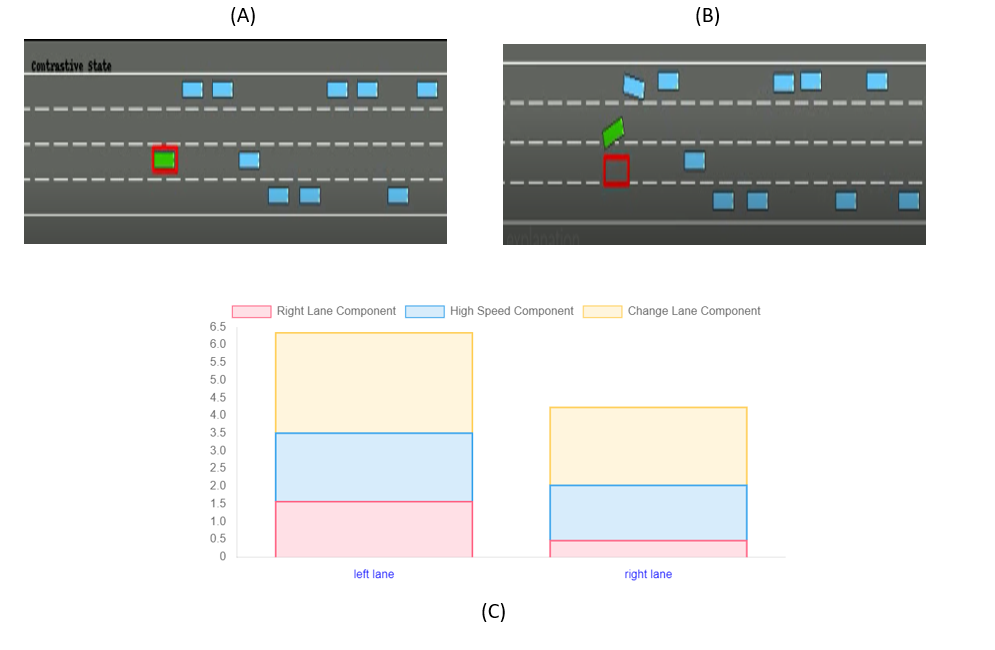
\includegraphics[scale=0.5]{figures/survey_example.PNG}
% \caption{Screenshots from the survey where (A) represents the contrastive state in the video. (B) shows the last frame of the scenario shown in the video, and (C) presents the reward bar for the state shown in (A)}
% \label{fig:survey_example}
% \end{figure}

\subsection{The Highway Environment}
\label{sec:Highway_env}
In the highway environment (see Figure \ref{fig:highway environment}) the RL agent controls a green vehicle that navigates a multi-lane highway while driving alongside and interacting with other (blue) vehicles. The agent can choose to accelerate, decelerate and change lanes. The environment can be modified for the number of lanes, vehicle speed range, the number of vehicles, vehicle density, and more.

We chose the highway domain since there is no clear “optimal” behavior, as there is no inherent goal that must be reached. The agent's reward is determined by its driving regime, therefore, it is possible to design agents with varied, reasonable strategies. Additionally, it is both easily understandable to lay users, and represents a relatable real-world scenario.

We focus on a single domain in the current study, as both reward decomposition and approaches similar to contrastive highlights (e.g., HIGHLIGHTS, DISAGREEMENTS) have been shown to generalize to additional domains in prior work \cite{amir2018highlights,juozapaitis2019explainable,sequeira2020interestingness,amitai2021don}.

\subsection{Agent Training}
All agents received a negative reward of $-3$ for reaching a collision state. The reward function specified positive rewards with the following behaviors, which were modified to generate a set of diverse policies: changing lanes (CL), speeding up (SU), and driving in the right-most lane (RML)). To account for each positive reward type, the number of components in the reward decomposition was set to $|C|=3$.
%We trained the agents as described in Section \ref{sec:background}.
The network input is a state that is represented by an array of size 25 (5X5). The input layer is followed by two fully connected hidden layers of length 256. The last of these two layers are connected to the three heads we defined. Each head consists of a linear layer and outputs a Q-value vector of length of 5 that contains the q-value for each of the possible actions: moving to the left lane, idle, moving to the right lane, going faster, going slower. 

We trained the following agents:
\begin{itemize}
    \item Agent 1 - The highest reward for changing lanes, then for driving in the right-most lane, and lastly for speeding up.
    \item Agent 2 - The highest reward was for driving in the right-most lane, then for changing lanes, and lastly for speeding up.
    \item Agent 3 - The highest reward was for speeding up, then changing lanes, and lastly being in the right-most lane. 
  \end{itemize}

No future rewards are obtained upon ending the episode. We experimented with different reward type values to get qualitatively different agent behaviors. The precise values for the agent configurations used in the user studies are summarized in Table \ref{tab:reward setting}.
Each agent was trained for 2,000 episodes and each episode consists of 80 steps (or fewer if the agent crashed). 

Our implementation is based on two open-source repositories: the Highway environment and an implementation of double DQN \cite{highway-env,rl-agents}.


To extract the contrastive highlights, we ran 1,000 simulations of the trained agents and saved their traces. The summary states extracted from these traces were used in the study.

\begin{table}
    \centering
    \begin{tabular}{|c|c c c |}
        \hline
        Reward Type  & CL  & SU & RML  \\
           % & reward & reward& reward \\
        \hline
        Agent 1 & 3 & 1 & 8  \\
        
        Agent 2 & 5 & 8 & 1  \\
         
        Agent 3 & 8 & 1 & 5 \\
        
        \hline
        
    \end{tabular}
    \caption{The reward type values of study highway environment agents.}
    \label{tab:reward setting}
        \vspace{-0.3cm}

\end{table}

\begin{figure}
\centering
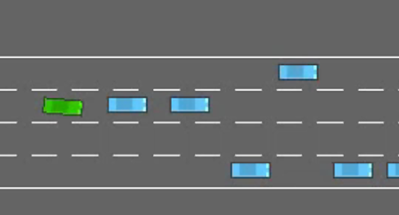
\includegraphics[width=0.8\linewidth]{figures/Highway_env2.png}
\caption{The highway environment}
\label{fig:highway environment}
\end{figure}

\begin{figure}[t]
\centering
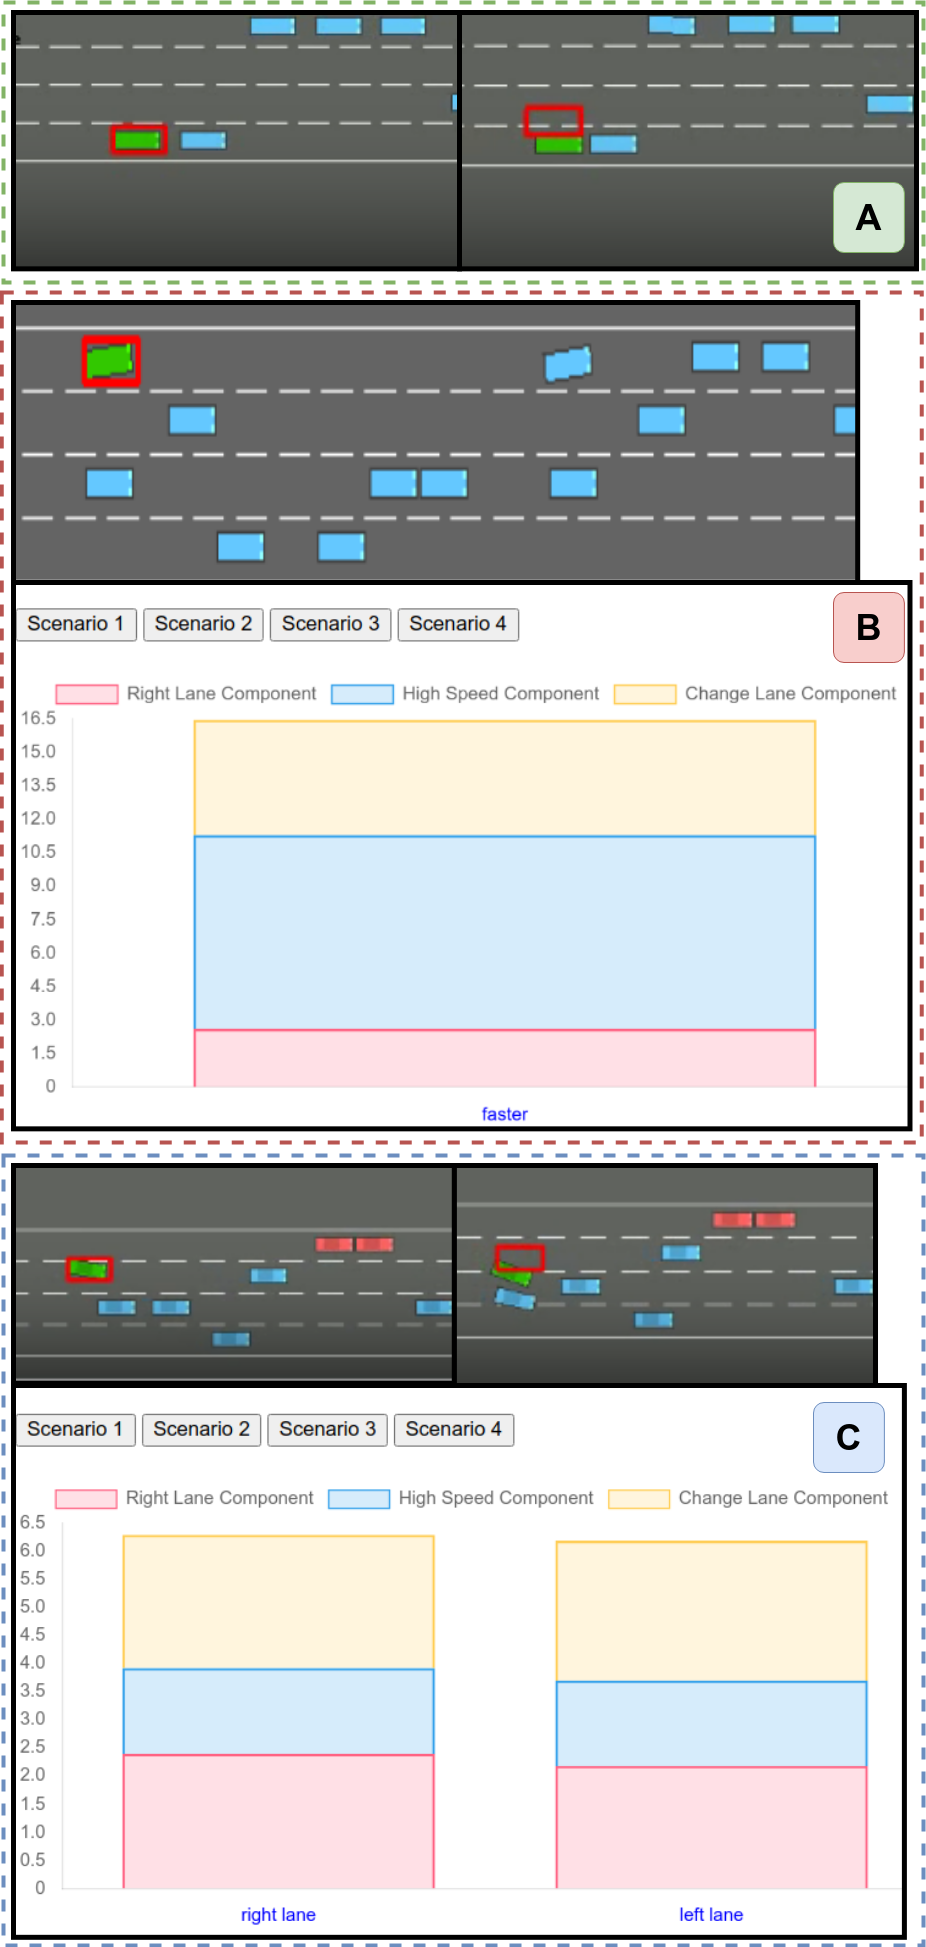
\includegraphics[width=0.9\linewidth]{figures/exp_types.PNG}
\caption{Examples of user study explanation types. \textbf{A. Contrastive Highlights (CH)}: videos depicting the different outcomes of contrastive actions; \textbf{B. Reward Decomposition (RD)}: a graph denoting the value each reward component contributed at the portrayed state; \textbf{C. Integrated method (CRD)}: The CH outcome video and a graph of both the chosen and contrastive action.}
\label{fig:exp_types}
\end{figure}

\subsection{Study Design}
We conducted two studies to evaluate the contribution of contrastive highlights and its integration with reward decomposition to people's understanding of agents' preferences. Study 1 was a between-subject study, where each participant only saw one type of explanation. This design avoids learning effects, but suffers from higher variance due to differences between study participants. To address this limitation, study 2 used a within-subject design where each participant was exposed to all explanation methods, and could thus compare them directly.  Both studies were approved by our institutional review board.

\emph{Experimental conditions}. The studies included three types of explanations:  contrastive highlights (\textit{CH}), reward decomposition (\textit{RD}), and their integrated configuration (\textit{CRD}). Examples of all explanation types can be seen in Figure \ref{fig:exp_types}. In study 1, each participant was assigned to one of the conditions and saw information about each of the three agents using the same explanation method. 
In study 2, all participants saw all three agents in a random order, but each agent was accompanied by a different, randomly assigned, explanation type. The ordering of the \textit{CH} and \textit{RD} explanations was random, however, the integrated method was always shown last as it was more natural to show it after showing each method separately.

\begin{figure}[t]
\centering
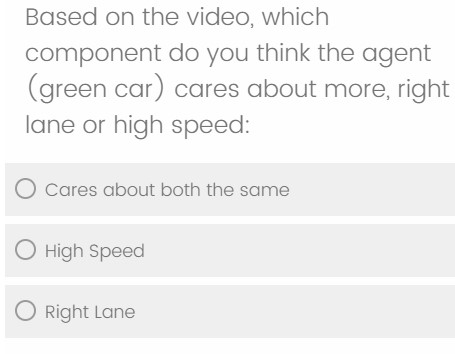
\includegraphics[width=0.7\linewidth]{figures/study_pref_question.jpg}
\caption{Example user study agent preference question.}
\label{fig:study_pref_question}
\end{figure}


\emph{Task.} 
In both studies, the participants' task was to assess the behavioral preferences of the different agents.
For each agent, participants observed four scenarios (i.e., states) and their explanations. The scenarios were chosen by the contrastive highlights algorithm which prioritizes states based on their ``importance'' value as described in section \ref{sec:ch_importance}. Since the Q-values of each agent are different, the ``important'' states differ as well. However, for a specific agent, all participants viewed the same scenarios. After participants observed the explanation of the agent's behavior in each scenario, they were asked to predict the agent’s preferences between two reward components (see Figure~\ref{fig:study_pref_question}), i.e., whether the agent prioritizes one of them or is indifferent between the two options. Participants could return and review the explanations while answering the questions.
The agents' order and the task answers were randomly presented. 

After each task participants rated their agreement on a 7-point Likert scale with the following items adapted from the explanation satisfaction questionnaire proposed by \cite{hoffman2018metrics}:
\begin{enumerate}
\item The videos$\backslash$graphs helped me recognize agent strategies
\item The videos$\backslash$graphs contain sufficient detail for recognizing agent strategies
\item The videos$\backslash$graphs contain irrelevant details 
\item The videos$\backslash$graphs were useful for the tasks I had to do in this survey
\item The specific scenarios shown in the videos$\backslash$images were useful for the tasks I had to do in this survey.
\end{enumerate}
Then, participants were asked to rate their confidence in each of their answers on a Likert scale from 1 (``not confident at all'') to 5 (``very confident'') and they had the option to describe their reasoning in a free-text response.

In study 2, since participants saw all three explanation types, they were also asked to rank their preferences among them and provide textual feedback regarding how each method helped them.

\emph{Procedure.} In both studies, participants were first introduced to the highway environment. Then, participants learned about their condition's explanation method along with an example to assist in interpreting the visualized information. In study 1, participants were presented with only one of the three explanation types: \textit{CH}, \textit{RD}, or \textit{CRD}. The explanation type was randomly assigned and  consistent across all three tasks.
Before each task, in study 2, instructions and information regarding the upcoming explanation method were initiated, after which, a demonstration was provided for the task they would be asked to complete.
Prior to starting the task itself, participants were quizzed on their understanding and only allowed to proceed once answering all questions correctly. Each task included an attention check question. Finally, participants were asked to provide demographic information and rate their proficiency in AI.
All study materials including the specific instructions for each explanation method can be found in the supplementary.

\emph{Participants}. We recruited participants through Amazon Mechanical Turk ($N=90$, and $N=50$ for study 1 and study 2, respectively). On average, study participants had low proficiency in AI which aligns with the purpose of explanations for laypeople. Participants were native English speakers, ages 18 - 55 from the US, UK, or Canada.
Participants received a \$3 base payment and an additional bonus 30-cent bonus for identifying the preferences of each of the agents correctly. Participants who failed the attention question were excluded from the final analysis, as well as participants who completed the survey in less than two standard deviations of the mean completion time. Eventually, study 1 consisted of 88 participants (divided as follows: CH=30, RD=31, CRD=27) and 49 participants in study 2 with a mean age of 39 \& 37, and a female count of 39 \& 27 for study 1 and 2 respectively.


\begin{figure}[t]
\begin{minipage}{0.49\linewidth}
\centering
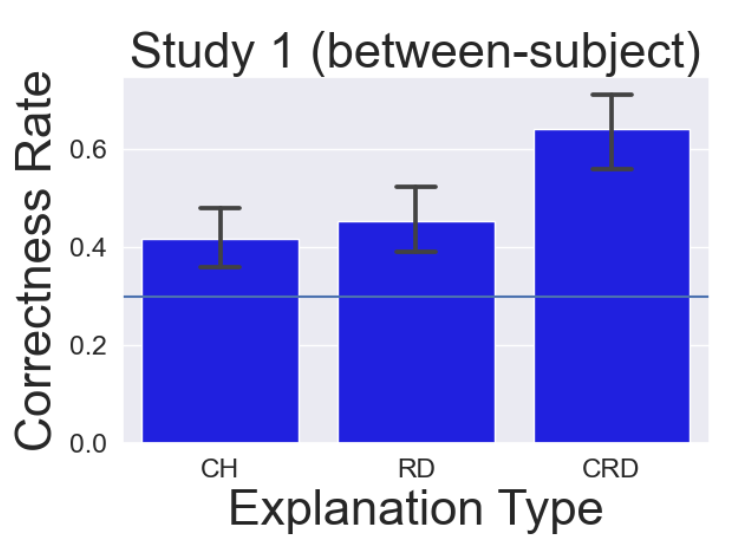
\includegraphics[width=\linewidth]{figures/First_study_correction_rate.PNG}
(A)
\end{minipage}
\begin{minipage}{0.49\linewidth}
\centering
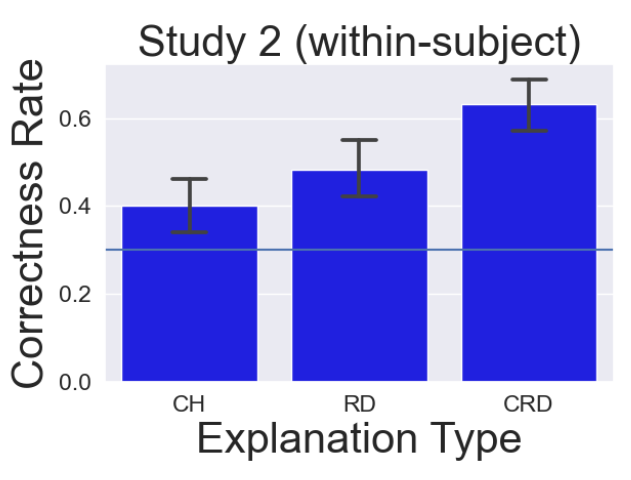
\includegraphics[width=\linewidth]{figures/Second_study_correction_rate.PNG}
(B)
\end{minipage}
\caption{Participants' mean success rate in identifying the preferences averaged over all agents by conditions in Study 1 (A) and in Study 2 (B). The error bars show the 95\% CI. }
\label{fig:results}
    \vspace{-0.2cm}
\end{figure}

\section{Results}
The objective measure used in our analysis is the  mean fraction of correct reward component comparisons, i.e., participants' correctness rate, for each condition. We used the non-parametric Mann-Whitney $U$ test in the statistical analyses.

Overall, the integration between the two explanation types improved participants' ability to asses the agents' preferences.
% To measure this ability, we calculated the mean fraction of correct reward component comparisons, i.e., their correctness rate, for each condition.
These results were replicated in both studies, and are summarized in Figure~\ref{fig:results}. 
In study 1, the integration method of combining both explanation types CRD (\textit{M}= 0.64) led to significantly improved performance compared to  RD or CH alone (RD: M=0.45, RD vs. CRD: $U=204,p<0.001$; CH: M=0.42, CH vs. CRD: $U=657.5, p<0.001$). The difference between CH and RD was not significant ($p = 0.22$).
Similarly, in study 2, the combination of the two explanation types, CRD (\textit{M}= 0.63), significantly improved participants' performance compared to RD  or CH (RD: M=0.48,  RD vs. CRD: $U= 767, p<0.001$ and CH: M= 0.4,  CH vs. CRD: $U= 1814.5, p<0.001$).  Here too, the difference between CH and RD was not significant ($p = 0.064$).
% The feedback from participants' textual responses provides evidence that they indeed made use of both types of explanations and benefited from their complementary nature. % The video help with the choose to correct answer and graph also helped with the move this surway
% % The combination of both was very useful in this task.
% For instance, one participant wrote \textit{``The video helped ... choose [the] correct answer ... graph helped [understand] ... the movement this way''}




In study 1, when breaking down the results by agents, the trend of the results was consistent with the overall results. The greatest improvement from the integration of the two approaches was for Agent 1 (see Figure~\ref{fig:first_study_agent1}. We note that Agent 1 is a tricky agent  as its second preference - being in the right-most lane is correlated with its first preference changing lanes. This shows that the combination of the two explanations has a significant impact, especially for challenging behaviors. Participants' comments also mentioned the benefit of combining the different explanations. For instance, one participant wrote that ``The two [explanations] together helped me understand but separately I was a lot more confused''. Another comment was ``The graphs help to visualize how the agent is rewarded for behaviors while the videos show the results of rewarding (or prioritizing) those actions for the agent.''

In study 2, we asked participants to rank the three explanation types.
Participants differed in their preferences. Some preferred the video-based approach of contrastive highlights, e.g., ``video is always easy for me to comprehend'', while others preferred the reward bars: ``The graph is more efficient''. A participant that preferred the combination wrote: ``It is more instructive to both see the component values and then watch the video. ''
The overall ranking results show that contrastive highlights were ranked in the first place by 28  participants ($57\%$ of participants), while the combination of the two explanation types was ranked in last place by 26 participants  ($53\%$ of participants) as shown in Figure~\ref{fig:ranking}.

For both studies, participants' confidence and satisfaction ratings were above the neutral rating ($>3$). Specifically, for study 1 and study 2 the satisfaction results for each of the conditions were CH: M=4.9 and 5.16, RD: M=5.06 and 5.06, CRD: M=5.29 and 5.04, respectively (see Figure ~\ref{fig:satisfaction}). With respect to participants' confidence, the ratings by condition observed in study 1 ans 2 were CH: M=4.04 and 3.93, RD: M=3.8 and 4.02, CRD: M=4.03 and 3.83, respectively). None of the differences between conditions in terms of satisfaction or confidence were significant.



\begin{figure}
\centering
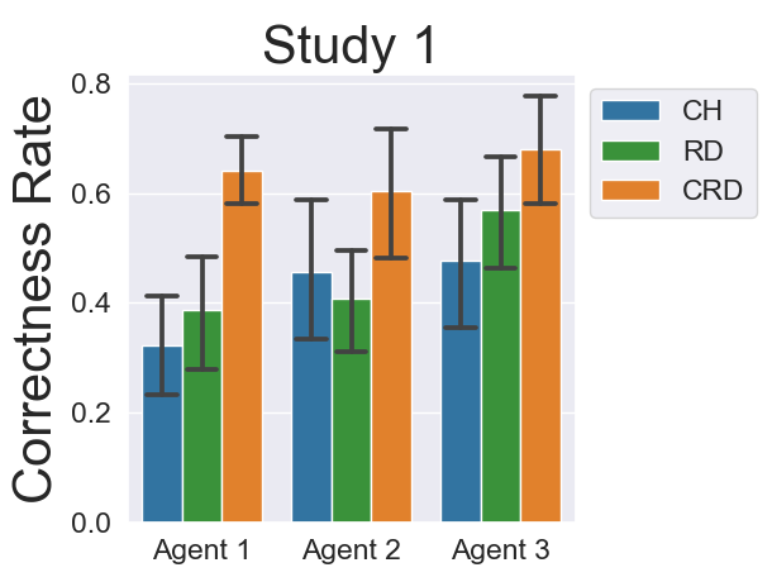
\includegraphics[width=0.7\linewidth]{figures/first_study_agent1.PNG}
\caption{Participants' mean success rate in identifying the preferences by condition and agent in study 1. The error bars show the 95\% CI.}
\label{fig:first_study_agent1}
    \vspace{-0.2cm}
\end{figure}



\begin{figure}
\centering
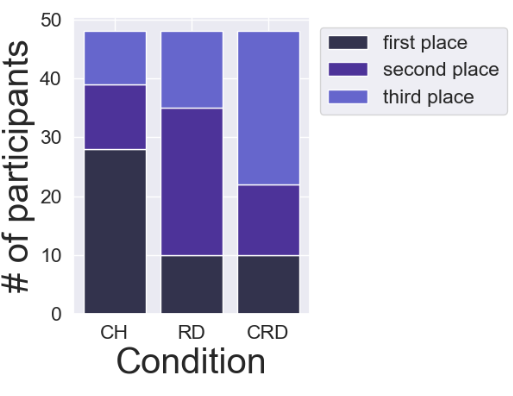
\includegraphics[scale=0.5]{figures/ranking_by_condition.PNG}
\caption{The distribution of participants' ranking of the three explanation types}
\label{fig:ranking}
\end{figure}


\begin{figure}[t]
\begin{minipage}{0.49\linewidth}
\centering
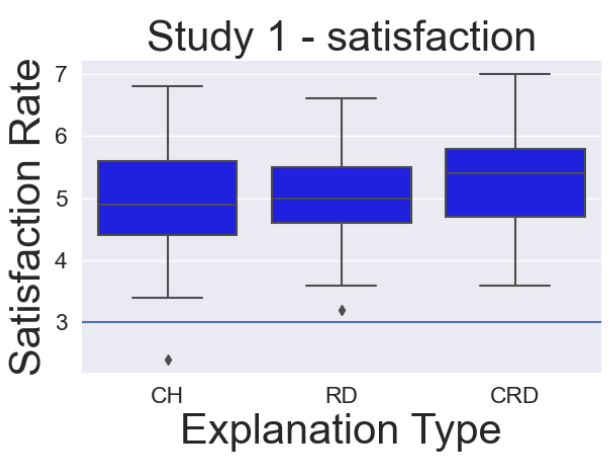
\includegraphics[width=\linewidth]{figures/satisfaction_first_study.PNG}
(A)
\end{minipage}
\begin{minipage}{0.49\linewidth}
\centering
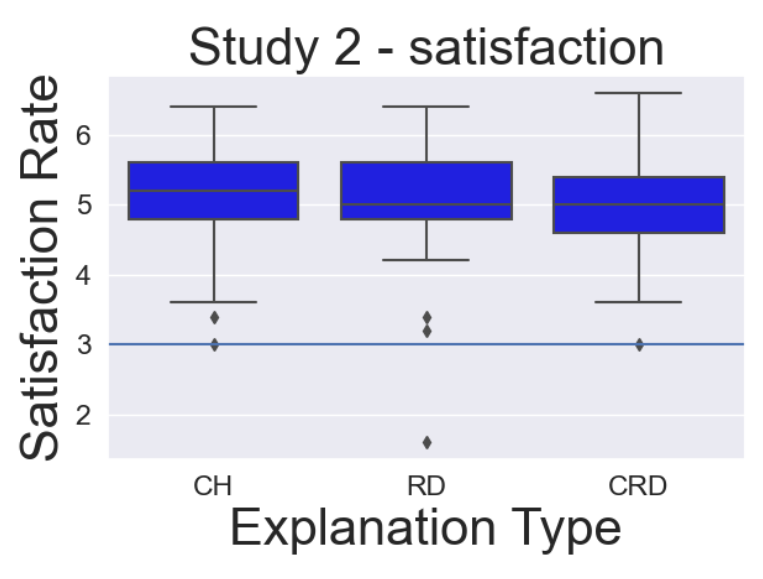
\includegraphics[width=\linewidth]{figures/satisfaction_secound_study.PNG}
(B)
\end{minipage}
\caption{Participants' satisfaction rate aggregated over all agents by conditions in study 1 (A) and in study 2 (B).}
\label{fig:satisfaction}
    \vspace{-0.2cm}
\end{figure}

\section{Discussion and Future Work}
This paper presented a new method for explaining RL agents - contrastive highlights, and the benefit of combining this local explanation with another local explanation - reward decomposition. We conducted two user studies to evaluate the contribution of this approach to people's ability to analyze agent preferences as well as rating the participants' preferences of each explanation type. Our results show that each of the explanation types, contrastive highlights, and reward decomposition, resulted in participant performance that is better than random guessing on its own, but the integration of the two methods enabled participants to reach a significantly higher success rate. It is not trivial that this would be the case since the benefit might only stem from one explanation, and the cognitive load might be higher as was observed in some studies~\cite{anderson2020mental}.


Even though the combination of the explanation types led to a higher correctness rate, when participants were asked to rate the explanation types, the combination was ranked last. We hypothesize that the reason for that is the mental overload on the participants. For example, one participant commented that ``...the combination is too confusing for me.''
When combining two explanation types participants are required to pay attention to more details. This finding is also in line with other works that show that subjective satisfaction and proxy tasks often do not align with objective performance ~\cite{buccinca2020proxy}.

Furthermore, the selection of ``important'' states, which was used in this study based on the last state importance, can be considered as a global explanation. The criteria for selecting which states to show can easily be changed, and various alternative criteria were proposed in the literature~\cite{lage2019exploring,huang2019enabling}. In addition, while here the choice of important states was guided by the contrastive trajectories, it is also possible to devise criteria that are based on reward decomposition, such as presenting states where different reward components are dominant. The approach can also be used to show a local explanation for a world-state chosen by the user. The use of this approach for different sets of world-states can be explored in future work.

Finally, while this work focused on the task of identifying agent preferences, future work can try to characterize which explanation types are most useful for different user tasks, and explore the combination of other local explanation types, including saliency maps, action graphs, and others.

\bibliography{bib}
\end{document}
%%%%%%%%%%%%%%%%%%%%%%%%%%%%%%%%%%%%%%%%%%%%%%%%%%%%%%%%%%%%%%%%%%%%%%
